\begin{figure}[h!]
	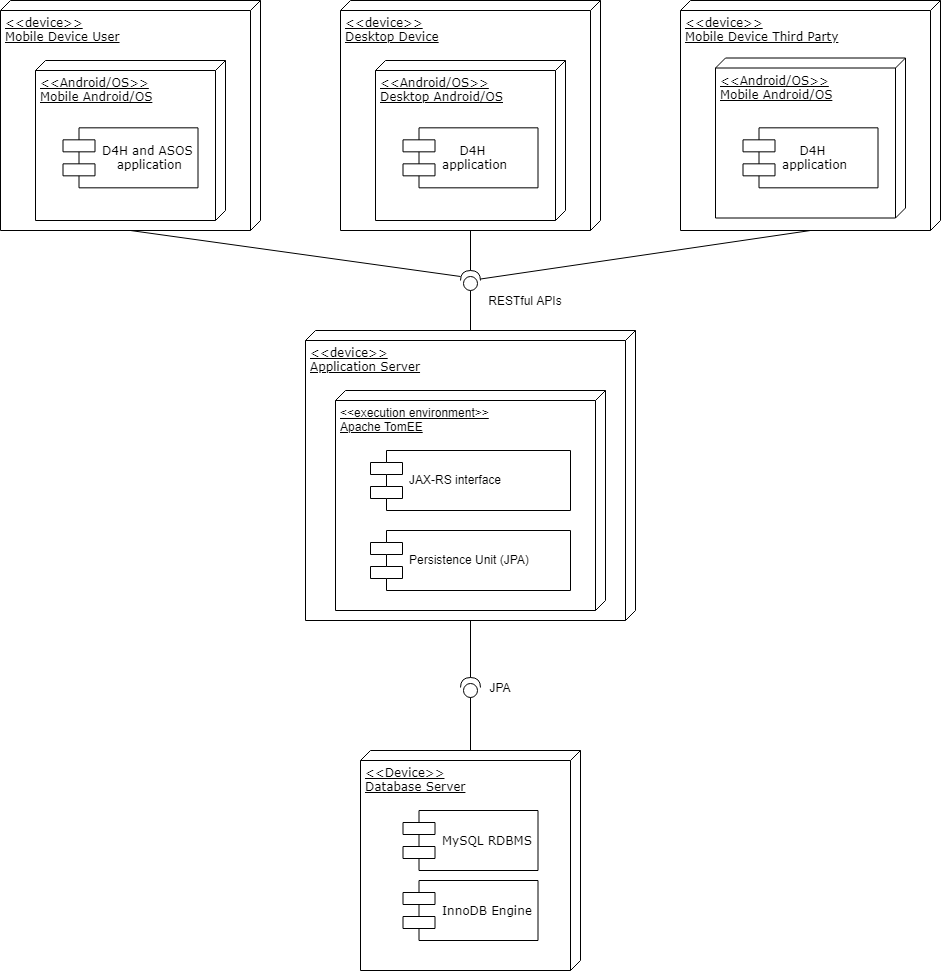
\includegraphics[width=1.0\textwidth]{./pictures/deployment_diagram.png}\par
	\caption{Deployment diagram}
\end{figure}
\FloatBarrier The Mobile App of users and third parties must be available on both IOS and Android systems; in order to obtain it the presentation layer must be code in Java for Android and in Swift for IOS.\\
In the diagram it is possible to find some implementation choices which are analyzed in the following lines.\\
It has been choice to use Java Enterprise Edition 8.2 (JEE) for the app layer because the aim of the final product is to become a large scope application with a great number of simultaneous clients and because, thanks to the ammount of APIs and tools the developers can focus on the main logic.
Here there are some choices made for the App Server implementation:
\begin{itemize}
	\item TomEE has been choice as server because it is an incredibly lightweight app, in fact it offers only the most basic 				functionality necessary to run a serverand it allows to use other API to solve all non basic ones. Thanks to its lightweight it is 			quite flexible and stable. TomEE has been choice also because it has born as a Web Server and than it became something close to 		an application server; for this reason it is totally compatible also with the 3 layer architecture that has been proposed in this 			document.
	\item The RESTful APIs architecture is applied because it makes the efficiet use of the bandwidth and uses standard HTTP. It 			also has a great scalability and it allows to carry out basic operations;
	\item JAX-RS to implement proper REStful APIs to interface with clients;
	\item Java Persistence API (JPA) as persistence Unit to acces the database. It has been picked out because it is an Object/			Relational Mapping (ORM) framework applicable to RDBMS without implement direct SQL queries and because of its high 				performances , scalability, stability and quality.
\end{itemize}
The DB's implementation choices are the following:
\begin{itemize}
	\item JPA within the App Server as the interface to the DB;
	\item MySQL as the RDBMS;
	\item InnoDB as the data engine; this is already the default engine applied to every table generated in MySQL but it has been 			choice because it associates high performances to high data consictency and integrity. To let this happens, this particular 			engine has developed some particular functionalities such as the introduction of foreign keys; locks at row level; Multiversion  			Concurrency Control (MVCC) to increment the concurrency in queries and support in tansactions to guarantee correctness in data.
\end{itemize}

\begin{figure}[h!]
	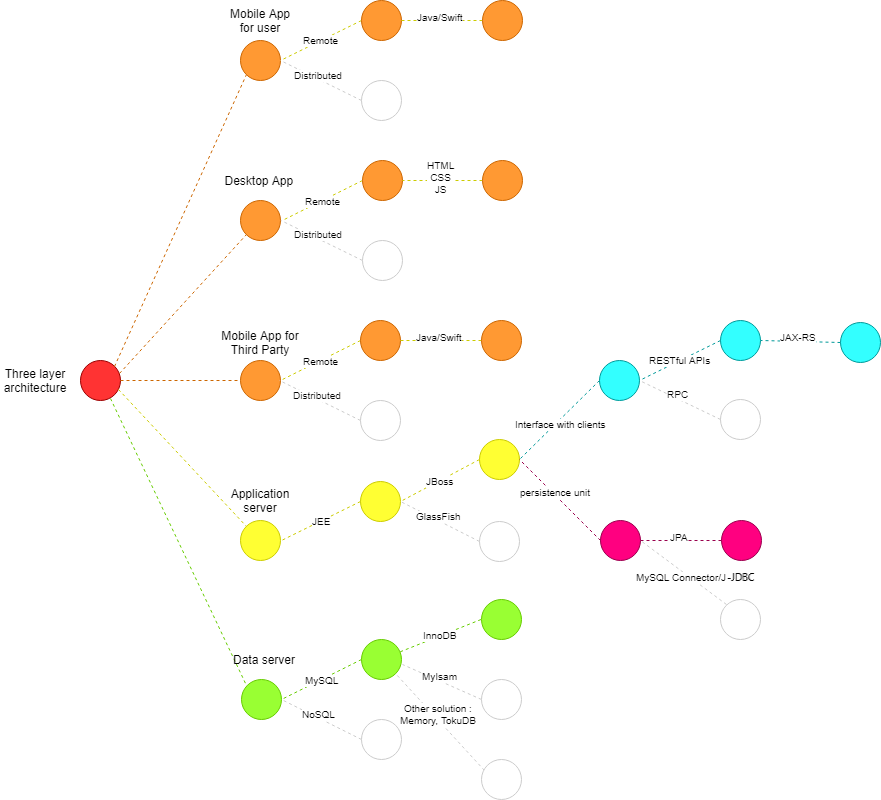
\includegraphics[width=1.0\textwidth]{./pictures/choice_diagram.png}\par
	\caption{The aim of this figure is to show which implementation possibilities have been discarded.It represents the decision 			tree for the starting architectural design. }
\end{figure}
\FloatBarrier
